\documentclass[../report]{subfiles}
\setcounter{section}{0}
\begin{document}

本章では,システム案出しのプロセスについて説明する.
\bunseki{山根春貴}

\section{システム案出し}
知識習得を経て,グループメンバーそれぞれが認知症に関する異なる分野の問題に着目してシステム案を考えた.その結果,「排泄通知システム」,「MyGO!」,「介護者SNS」,「認知症患者の見守りとプライバシーの両立」,「暴力・暴言行動記録システム」の5案が出た.アイデアの概要を以下で紹介する.
\bunseki{山根春貴}

\subsection{排泄通知システム}
これは家庭内の介護者(特に家族)を対象とし,認知症の人の排泄時間を事前に通知するシステムである.具体的には,排泄を行った時間を日々記録し,排泄予測時間前に通知をする.また,記録されたデータを利用すると,より精密な時間に通知できるようになると予測される.記録は便座に圧力センサを導入し,座ったときにセンサが反応し,デバイスに自動で記録してくれる.通知はPepperが音声で行う.
\bunseki{山根春貴}

\subsection{MyGo!}
これは軽度認知障害者を対象とした散歩支援システムである.手軽に撮れるライフログカメラを使用する.また,歩数計を用いることで使用者が意識せずとも使える.そのほかに,ウォーキングマップの情報を基にした散歩支援システムの機能を提案する.具体的に,五稜郭公園に入った時に見どころを音声で知らせる.クイズを出してクイズに成功するとスタンプなどの報酬を得られる,などの機能を導入する.
\bunseki{山根春貴}

\subsection{介護者SNS}
これは認知症患者の介護者を対象とした介護者同士での意見交換ができる場をつくるシステムである.認知症患者の介護者(家族,ヘルパー),そして地域の認知症サポーターが参加するSNSである.介護者の悩み相談,認知症に関する知識共有ができる.認知症患者の情報をあらかじめ非公開で登録しておき,行方不明時に周囲数km内の他のユーザーに通知される.
\bunseki{山根春貴}

\subsection{認知症患者の見守りとプライバシの両立}
これはグループホームのケアスタッフを対象としたシステムである.カメラを利用した見守りシステムにおけるプライバシ問題の解決と介護者の負担の更なる軽減を目的としている.カメラを用いた見守りシステムは,介護の現場における人手不足問題とさり気ない介護・観察の実現に効果が期待されるが,同時にプライバシ問題も抱えている.それを解決すべく,ICタグや画像分析等を利用することで,特に注意が必要な場所や場面の映像を選択的に介護者に提供する.
\bunseki{山根春貴}

\subsection{暴力・暴言行動記録}

\bunseki{山根春貴}


\section{システム案レビュー}
\subsection{指導教員からのレビュー}
2017年5月26日,指導教員からシステム案出しで出たシステム案のレビューを頂いた.
頂いたレビューの一部を以下に紹介する.
\begin{enumerate}
    \item 排泄通知システム
        \begin{itemize}
            \item 排泄感知装置をつけるのは嫌がりそう.
            \item 記録をするときデータの入力はどうするのか?
        \end{itemize}
    \item MyGo!
        \begin{itemize}
            \item 大枠としては良い.自由に散歩できることは認知症患者にこんな良い点がある,というアピールが必要である.自由に徘徊できる街,という事例がある\cite{haikai}.
            \item 症状に合わせたシステムの提案である必要がある.
        \end{itemize}
    \item 介護者SNS
        \begin{itemize}
            \item 既存のアプリとの違い,利点等を説明に入れると良いかもしれない.
            \item 函館市の話では,徘徊者を見つけたらすぐに警察に報告することになっている.
        \end{itemize}
    \item 認知症患者の見守りとプライバシーの両立
        \begin{itemize}
            \item プライバシーの危機を感じているのは患者か?対象者はどうなのか?
            \item 介護者が働きにくいと思う環境から,介護者をハッピーにするシステムにしてほしい.
        \end{itemize}
    \item 暴力・暴言行動記録システム
        \begin{itemize}
            \item 最終的な目的は暴力・暴言を減らすことなのか,暴言暴力に強くなることなのか?
            \item 暴力・暴言に対してのノウハウを家族に伝えるために記録して蓄積・統計を取るというのはどれくらいの効果があるのか?
        \end{itemize}
\end{enumerate}
\bunseki{山根春貴}

\subsection{函館認知症の人を支える会の代表者からのレビュー}
2017年5月31日,公立はこだて未来大学で行われた認知症サポーター養成講座を受講した.この講座では,認知症患者との接し方などの知識習得,自分たちで考えたシステム案に対するレビューを頂くことを目的として受講した.講師の方や教員から頂いたレビューの一部を以下に紹介する.
\begin{enumerate}
    \item 排泄通知システム
        \begin{itemize}
            \item 食事水分のとり方によって変わる.
            \item 年寄りは回数が増える.しかし介護者のストレスを軽減する良いアプローチだと思う.
        \end{itemize}
    \item MyGo!
        \begin{itemize}
            \item 最初のきっかけを与えるということを考えて欲しい.
            \item 万歩計の歩数に応じて何か還元できるものがあれば対象者も積極的にやってくれるようになるのでは?
        \end{itemize}
    \item 介護者SNS
        \begin{itemize}
            \item この考え方はすでにある.地域の助け合いネットワークとしては効果がある.地域ネットワークの中で,協力し合うとかだと発見に近くなる.
            \item 介護者SNSのような考え方は普段は写真を使わない.だから使うとなると効果は出ると思う.でも本人や家族の了解なしでやるのはどうだろうか.
        \end{itemize}
    \item 認知症患者の見守りとプライバシーの両立
        \begin{itemize}
            \item 実際にカメラが入っているグループホームがあるのか?認知症患者側が嫌だという論文はなくて,介護している側が嫌だという論文があったのか?
            \item 見守りとプライバシーは相反することである.徘徊を防ぐのであれば出口ぜんぶ閉じる必要がある.グループホームを出てしまうと難しい.どういうところを見守るかを明確にしないと考えまとまらないのではないと思う.
        \end{itemize}
    \item 暴力・暴言行動記録システム
        \begin{itemize}
            \item 暴力・暴言はパターン化出来ないと思う.問題は接し方である.それをグラフ化,何か作るというのはなかなか難しい.フィードバックもいつも同じものではない.家族の人間関係にもよる.一番難しい分野だと思う.
        \end{itemize}
\end{enumerate}
\bunseki{山根春貴}

\subsection{京都府立医科大学成本医師からのレビュー}
2017年6月7日,京都府立医科大学の成本医師とSkypeによる会議を行った.この会議では,システム案に対してのご意見を頂いたり,成本医師の要望を聞いたりした.会議で成本医師から頂いたご意見と成本医師の要望の一部を以下に紹介する.
\begin{enumerate}
    \item 排泄通知システム
        \begin{itemize}
            \item 健常者は日中にトイレに行き,夜は寝るだけという生活リズムをする.老いてくると夜もトイレに行くようになる.こういった排泄のリズムを録ることができれば良い(高齢化に伴う排泄のリズムの変化を見つける).生活の中にどれだけ自然な形でインストールするか,というのが重要である.
        \end{itemize}
    \item MyGo!
        \begin{itemize}
            \item 函館のウォーキングマップに沿った形で良いアイデアだと思う.ロボホンを首からかけて移動するとクイズを出したり,案内したり,というのは少し似ている.これはスマホをぬいぐるみに入れるというのでも代用できる.高齢者の方と一緒に歩いて,あとで振り返れると良い.
        \end{itemize}
    \item 介護者SNS
        \begin{itemize}
            \item 介護者特有の悩みを共有するできる場にする.
            \item 行方不明の通知は先行研究などで色々やられていて,いざというときだけ公開するのは良い.
        \end{itemize}
    \item 認知症患者の見守りとプライバシーの両立
        \begin{itemize}
            \item ケアの負担軽減,というのは日本でかなり必要とされている技術である.様々なものが作られているが,全然導入されていない.導入されていない理由の一つに認知症患者やスタッフの機械アレルギーがあり,現状のグループホームのシステムで満足してしまっている.
        \end{itemize}
    \item 暴力・暴言行動記録システム
        \begin{itemize}
            \item 暴力・暴言も施設入居のきっかけになる.行動療法は患者の行動を見て,療法を提示するが,今はアナログである.これをアプリ化すればより便利になるのではないかと思う.
            \item やはり可視化するというのは非常に重要である.記録することで,自覚しているしんどさと実際に起きていることが違ったりする.記録するだけで問題が解決することもある.いかに簡単に記録してもらうかということが重要だと思う.
        \end{itemize}
   \item 成本医師からの要望
        \begin{itemize}
            \item 医療選択における意思決定問題を支援できるようなシステムを考えてほしい.
            \item 映像だったり普段の何気ない選択などが可視化されて医療従事者に提供されると良いと思う.普段の傾向をつかむことやプロセスの透明化というのは医療選択する手段であるが,これをICTの力でアシストしてほしい.
        \end{itemize}
\end{enumerate}
\bunseki{山根春貴}

\subsection{もの忘れカフェでのレビュー}
2017年6月17日,函館総合福祉センターで行われたもの忘れカフェに参加した.このイベントでは,施設のことや認知症患者に詳しい方にシステム案を提案し,レビューを頂いた.時間の都合上,「排泄通知システム」と「MyGO!」の2案だけ提案した.もの忘れカフェで頂いたレビューの一部を以下に紹介する.
\begin{enumerate}
    \item 排泄通知システム
        \begin{itemize}
            \item 排泄や食事などの記録をとる期間は相当かかるのではないか?
            \item トイレに行った記憶がなくなって,トイレに行きたいという人もいる.
        \end{itemize}
    \item MyGo!
        \begin{itemize}
            \item ロボットを使うことについて,認知症患者の方がしゃべる→録音→すぐ再生する,というシステムがあった.最初は重度の認知症患者の方でも興味を示していたが,そのうち全く興味を示さないようになった例がある.
        \end{itemize}
\end{enumerate}
\bunseki{山根春貴}


\section{システム案の再検討}
\subsection{新しいシステム案}
頂いたレビューや知識習得からシステム案の改善を繰り返してきた.しかし,どのシステム案もいくつか問題点が残るものとなり,アイデアの試行錯誤が続いた.そこで,今までの案から建設的なアイデアが生まれることを期待して,案の再考という流れに至った.再考するまでのシステム案は,認知症患者やその介護者に関する問題を解決するシステム案を考えていたが,違う視点でアイデアを考えた.認知症になる前段階の高齢者を対象とし,4.2.3に記述した「映像だったり普段の何気ない選択などが可視化されて医療従事者に提供されると良い」という成本医師からの要望を参考にシステム案を考えた.システム案を考え,グループで出た方向性を以下にまとめた.
\begin{itemize}
    \item 認知症ではない高齢者の認知症のリスクを減らす
    \item ライフログデータを活用したコミュニケーションや生活習慣の見直しの切っ掛け作りをする
\end{itemize}
この方向性を整理してまとまった案が「認知症予防のための食習慣改善システム」である.運動や睡眠といった生活習慣の中で食習慣に着目した理由は,植木(2005)の調査から健常者と比較して,アルツハイマー型認知症患者の食生活バランスが崩れていることが明らかになっている[2]からである.システムのイメージ図を以下\ref{fig:sys-image}に示す.
\begin{figure}[htbp]
    \begin{center}
        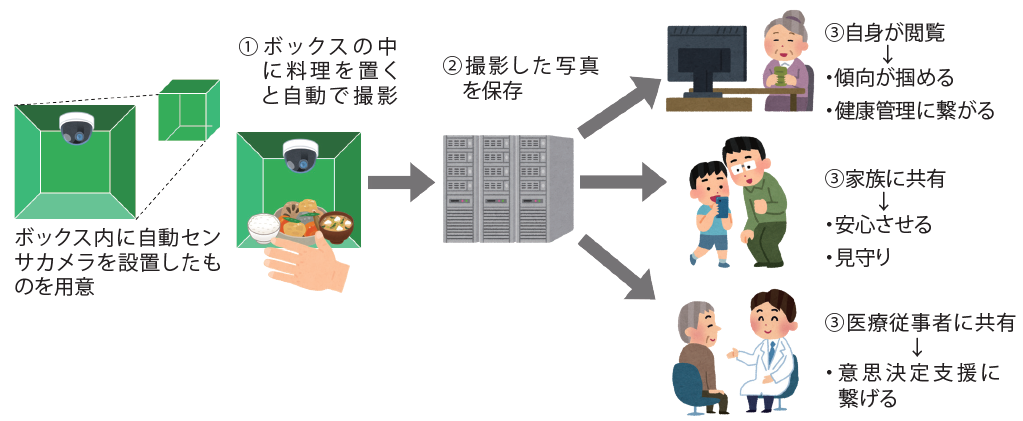
\includegraphics[width=10cm]{imgs/system-overview.png}
        \caption{システムのイメージ図}
        \label{fig:sys-image}
    \end{center}
\end{figure}
\bunseki{山根春貴}

\subsection{新しいシステム案に対するレビュー}
プロジェクト学習中に行われたレビュー会や中間発表会で「認知症予防のための食習慣改善システム」に対するレビューを頂いた.「意思決定支援につながった例はあるのか」といった先行研究についての質問や高齢者自身の閲覧のデータの見せ方,料理の撮影方法について多くのレビューを頂いた.
\bunseki{山根春貴}

\end{document}
